%%%%%%%%%%%%%%%%%%%%%%%%%%%%%%%%%%%%%%%%%%%%%%%%%%%
%% P3: Phenomenology of Particle Physics                         
%%
%% Author:  André Rubbia                   		 
%%
%% Figure 21.3 Crossing symmetry relates beta decay, electron capture, and inverse beta decay.
%%
%% This work is licensed under the Creative Commons Attribution 4.0 International License. 
%% To view a copy of this license, visit http://creativecommons.org/licenses/by/4.0/ or 
%% send a letter to Creative Commons, PO Box 1866, Mountain View, CA 94042, USA.
%%
%%%%%%%%%%%%%%%%%%%%%%%%%%%%%%%%%%%%%%%%%%%%%%%%%%%

\documentclass[a4paper,10pt]{article}

\usepackage[T1]{fontenc}
\usepackage[utf8]{inputenc}
\usepackage{lmodern}
\usepackage[labelfont=bf]{caption}
\usepackage{upgreek}

\usepackage{tikz}
\usetikzlibrary{patterns}
\usetikzlibrary{decorations.pathmorphing}
\usetikzlibrary{decorations.markings}
\usetikzlibrary{arrows}
\usetikzlibrary{svg.path}
\usetikzlibrary{shapes}
\usetikzlibrary{arrows.meta}
% define the arrow style
\tikzset{
    arrow/.style={
        decoration={
            markings,
            mark=at position .5 with {
                \arrow[#1, scale=1.5]{latex}
            }
        },
        postaction={decorate},
    }
}
\tikzset{
    arrow flipped/.style={
        decoration={
            markings,
            mark=at position .5 with {
                \arrow[#1, scale=1.5]{latex reversed}
            }
        },
        postaction={decorate},
    }
}
\usepackage{pgfplots}
\pgfplotsset{compat=1.17}
\usepgfplotslibrary{ternary}
\usepgfplotslibrary{fillbetween}
\usepgfplotslibrary{external}

\def\d{\mathrm{d}}
\setlength{\oddsidemargin}{-1.0cm}
\setlength{\evensidemargin}{-1.0cm}
\setlength{\textheight}{25cm}
\setlength{\textwidth}{18cm}

\begin{document}

%%%%%%%%%%%%%%%%   FIGURE  %%%%%%%%%%%%%%%%%%%%%%%%%%%%%%
\begin{figure}[htb]
\begin{center}
\begin{tikzpicture}

\begin{scope}[shift={(0,0)}]
\node at (0,2) {\bf Neutron beta decay};
\node at (0,1.5) {$n\rightarrow p+e^-+\bar\nu$};
\draw[blue,thick,-{Latex[width=3mm]}] (-2,0) node [left] {$n$} -- (-1,0) ;
\draw[blue,thick] (-1,0) -- (0,0);
\draw[blue,thick,-{Latex[width=3mm]}] (0,0) -- +(30:1.5);
\draw[blue,thick] (30:1.5) -- +(30:0.5) node [right] {$p$};
\draw[thick,red,-{Latex[width=3mm]}] (0,0) -- (1.5,0) ;
\draw[thick,red] (1.5,0) -- (2,0) node [right] {$e^-$};
\draw[red,thick] (0,0) -- +(-30:1.0);
\draw[red,thick,{Latex[width=3mm]}-] (-30:1) -- +(-30:1.0) node [right] {$\bar \nu$};
\node at (-0.25,0.25) {$G_\beta$};
\end{scope}

\begin{scope}[shift={(6.,0)}]
\node at (0,2) {\bf Electron capture};
\node at (0,1.5) {$e^- + p\rightarrow n+\nu$};
\draw[blue,thick,-{Latex[width=3mm]}] (150:2) node [left] {$p$} -- +(-30:1) ;
\draw[blue,thick] (150:1) -- (0,0);
\draw[blue,thick,-{Latex[width=3mm]}] (0,0) -- +(30:1.5);
\draw[blue,thick] (30:1.5) -- +(30:0.5) node [right] {$n$};
\draw[thick,red] (-150:1) -- (0,0) ;
\draw[thick,red,-{Latex[width=3mm]}] (-150:2) node [left] {$e^-$} -- +(30:1.0);
\draw[red,thick,-{Latex[width=3mm]}] (0,0) -- +(-30:1.0);
\draw[red,thick,] (-30:1) -- +(-30:1.0) node [right] {$\nu$};
\node at (0,0.35) {$G_\beta$};
\end{scope}

\begin{scope}[shift={(12,0)}]
\node at (0,2) {\bf Inverse beta decay};
\node at (0,1.5) {$\bar \nu + p\rightarrow n+e^+$};
\draw[blue,thick,-{Latex[width=3mm]}] (150:2) node [left] {$p$} -- +(-30:1) ;
\draw[blue,thick] (150:1) -- (0,0);
\draw[blue,thick,-{Latex[width=3mm]}] (0,0) -- +(30:1.5);
\draw[blue,thick] (30:1.5) -- +(30:0.5) node [right] {$n$};
\draw[thick,red,{Latex[width=3mm]}-] (-150:1) -- (0,0) ;
\draw[thick,red] (-150:2) node [left] {$\bar\nu$} -- +(30:1.0);
\draw[red,thick] (0,0) -- +(-30:1.0);
\draw[red,thick,{Latex[width=3mm]}-] (-30:1) -- +(-30:1.0) node [right] {$e^+$};
\node at (0,0.35) {$G_\beta$};
\end{scope}

\end{tikzpicture}
\end{center}
\caption{Crossing symmetry relates beta decay, electron capture, and inverse beta decay.}
\end{figure}
%
%%%%%%%%%%%%%%%%   END FIGURE  %%%%%%%%%%%%%%%%%%%%%%%%%%%%%%
%
\end{document}
